\begin{graphicspathcontext}{{./chapters/mas/imgs/},{./chapters/mas/imgs/auto/},\old}

\begin{frame}{{Two perspectives} on Agent-based Systems}
	\begin{columns}
		\begin{column}{.5\linewidth}
			\centering
			\fancybox[width=7cm,bg=CIADdarkgray]{Mono-Agent Approach}{
				\Emph{System composed of a single agent} \\
				Example: personal assistant
			}{monoagent-system}{1}
		\end{column}
		\begin{column}{.5\linewidth}
			\centering
			\fancybox[width=7cm]{Multi-Agent Approach}{
				\Emph{System composed of multiple agents} \\
				Global or collective task is built from agent actions \\
				Result \emph{emerges} from the local interactions and behaviors
			}{multiagent-system}{+}
		\end{column}
	\end{columns}
\end{frame}

\begin{frame}{{Multiagent System:} a first definition}
	\begin{definitionblock}{Multiagent System \cite{Wooldridge09}}
	Multi-agent system is a system composed of multiple interacting intelligent agents, where each agent has incomplete information or capabilities to solve a problem and thus must interact with others to achieve its goals or the system's goals
	\end{definitionblock}
\end{frame}

\sidenote{Images by Claude Sonnet 4.6}
\begin{frame}{Interaction in Multiagent Systems}
	\begin{description}
		\item[Direct Interaction] \raisebox{-.4\height}{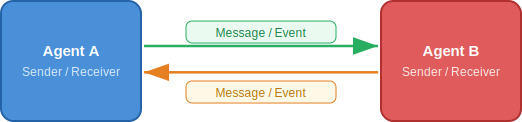
\includegraphics[width=.6\linewidth]{direct_interaction}}
		\vspace{.5cm}
		\item[Indirect Interaction] \raisebox{-.4\height}{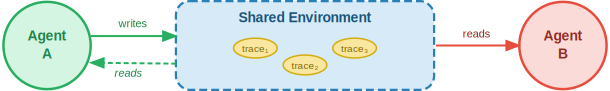
\includegraphics[width=.7\linewidth]{indirect_interaction}}
	\end{description}
	\begin{columns}
		\begin{column}[t]{.5\linewidth}
			\begin{definitionblock}{Stigmergy in biology \cite{Grasse59}}
				Form of self-organization in which the trace left in the environment by an action stimulates the performance of a subsequent action, either by the same entity or by other entities
			\end{definitionblock}
		\end{column}
		\begin{column}[t]{.5\linewidth}
			\begin{definitionblock}{Stigmergy in MAS \cite{Dorigo92}}
				Agents interact by modifying a shared environment and these modifications influence the subsequent actions of the same or other agents
			\end{definitionblock}
		\end{column}
	\end{columns}
\end{frame}

\begin{frame}{{Multiagent System:} another definition}
	\begin{definitionblock}{Multiagent System \cite{Ferber.1999}}
		System comprising the following elements: 
		\begin{itemize}
		\item An environment E, usually a space (may be with volume, 3D)
		\item An array of objects, $O$. These objects are situated
		\item A set of agents, $A$, which are specific objects
		\item A set of relations, $R$, which links the objects (and thus agents)
		\item A set of operations, $Op$, making it possible for agents to receive, produce, process and manipulate the objects in $O$
		\item Operators with the task of representing the application of these operations and the reaction of the world to this attempt of modification
		\end{itemize}
	\end{definitionblock}
\end{frame}

\begin{frame}[t]{Modeling from Local to Global}
	\vspace{-.25cm}
	\hiconbox{
		\Emph{Individual level:} design each agent model
		\begin{description}
		\item[Agent architecture] internal decision process based on reactive or proactive mechanisms
		\item[Autonomy level] delegate tasks to agent capacities, resources or the operating system
		\end{description}
	}{monoagent-system}
	\hiconbox{
		\Emph{Society level:} choose the global mechanisms
		\begin{description}
		\item[Hierarchy] is and how agent composed by other agent?
		\item[Decentralization] how control is distributed other agents, who has authority? (social pattern, norms)
		\item[Agreement technologies] how to coordinate, cooperate, negotiate?
		\item[Emergence] how to implement and influence emergence?
		\item[Distribution] how agents are physically distribued?
		\end{description}
	}{multiagent-system}
\end{frame}

\end{graphicspathcontext}

\endinput

